\chapter{绪言}
\label{chap1_introduction}
\section{研究背景}
随着科学技术的不断向前,人们对于工程应用中的设计可靠性和虚拟应用中的真实感体验亦在不断提出更高的要求。而物理仿真作为解决此类问题的关键技术手段,在计算机硬件的不断发展和计算能力大幅度提升的背景下,近年来得以快速跨越式向前发展。

所谓基于物理的仿真是指通过对物体建立能够表征其物理属性的动力学模型,在计算机上以某种合适的方式进行离散数值计算,从而能对真实世界中的物理行为进行模拟。物理仿真在计算机科学中占据重要地位,并应用于多个不同的关键领域。例如,在基础物理领域,往往通过物理仿真来寻找其中的统计规律,揭示真实世界中的物理原理。在计算机图形学领域以及电影、游戏等工业界,物理仿真更是给用户带来高逼真度沉浸式体验的关键技术。总之,物理仿真应用具备数据密集和计算密集双重特点,其作为一项基础性技术,在电影、工程设计、游戏等产业领域应用广泛、用户众多,是国家近年来大力发展的战略性新兴领域。

形变仿真是物理仿真的重要组成部分。形变现象在生活中几乎无处不在,常见的形变体材料包括人体的肌肉组织、布料、纸张、毛发、橡胶果冻等。事实上,绝对的刚体是不存在的,物体都或多或少存在一定形变。形变体的形变行为非常复杂:拉伸、压缩、扭曲等。在工程领域,碎裂仿真是研究材料特性以及进行辅助结构设计的重要手段。不过相对于工程材料等科学领域对于仿真精确性的高要求,图形学领域的应用相对更强调系统的稳定性和视觉效果。为提高效率,往往倾向于对模型进行一定的简化以更快地得到结果。

碎裂仿真是物理仿真的另一个重要分支。在日常生活中,碎裂效果(如玻璃碎裂、爆炸等)往往给人以深刻印象。碎裂仿真是游戏动画、数字电影和工程仿真等领域的研究热点,其具有极大的应用价值。在电影特效领域,出于成本以及人员安全的考量,真实地拍摄爆炸等大规模碎裂场景往往不具有可行性。而通过高性能计算机进行碎裂仿真,不仅能够降低电影的制作成本,而且可以控制整个断裂或者碎裂的过程,还有利于艺术家的后期设计与制作。在游戏领域,碎裂现象的实时模拟更是交互的重要组成部分,是给予玩家真实游戏体验的关键要素。在国防领域,因为炸弹轰击而产生的爆炸效果也是碎裂的一种典型现象,对于爆炸效果的碎裂仿真将极其有助于研究武器的杀伤力,进行武器的设计。弹塑性物体的碎裂在生活中也随时可见,如橡胶材料的碎裂等。手术时对人体器官的切割实际上也是一种形变体碎裂,研究在虚拟手术中的人体组织器官的交互式切割仿真,可在手术演示和手术人员的操作训练起到重要辅助作用,更具有广阔的前景。

虽然近年来,物理仿真已经在学术界得到广泛研究。但至今为止,尤其对于碎裂仿真,仍然缺乏能够在计算的效率上、计算的稳定性和可靠性上以及实现的简单性上能够支撑起工业界应用的仿真方法,更为成熟的形变仿真和碎裂仿真方法亟待进一步探索。本文的目的即是从近场动力学理论出发,提出了一整套用于弹塑性材料的形变、可延展性碎裂和脆性碎裂的无网格仿真框架,为物理仿真提供新的思路。

\section{相关工作综述}
\label{related_work}

\subsection{弹塑性形变仿真}

在图形学领域,最开始的塑性形变体仿真可以追溯到 \mycite{Terzopoulos}{1988}。随后 \textcolor{blue}{(O'Brien et al. 2002)\parencite{OBrien2002}} 在 FEM 框架中引入了一个加法形式的塑性模型来模拟可延展性材料的碎裂。在其模型中,应变张量被分解为两个部分:弹性形变和塑性形变。\textcolor{blue}{(M\"{u}ller et al. 2004)\parencite{Muller2004}} 同样采用这一模型用来模拟物体的塑性行为,但这一工作是在基于粒子的无网格框架进行的。随后\mycite{Irving}{2004}在其工作中提出了一个关于塑性的乘法模型,并指出其能更好的处理塑性行为。不同于加法模型,乘法模型是将形变分解相乘的两个部分。这一模型后续被其他工作广为采用,如\mycite{Bargteil}{2007}模拟大规模场景下的粘滞流体,\mycite{Gerszewski}{2009}仿真弹塑性固体,\mycite{Stomakhin}{2013} 用来模拟雪的塑性等。

然而上述几乎所有的办法几乎都无法直接应用于近场动力学模型,因为在其积分表述中并存在形变梯度或者应变张量的概念。因此,在本文我们将呈现一个全新的适用于近场动力学的塑性模型。不过,本文工作采用的塑性模型实际上同样为加法模型,在设计上亦一定程度上参考了\textcolor{blue}{(O'Brien et al. 2002)\parencite{OBrien2002}}。


\subsection{碎裂仿真}

近年来,在计算能力不断提升和人们对于真实度体验有更高需求的背景下,碎裂现象愈发成为虚拟游戏和电影等不同领域应用中不可或缺的一部分。碎裂仿真在工程和计算机图形学等领域已经得到广泛研究,并且在学术界提出了各式各样的算法,具体参见综述\mycite{muguercia}{2014} , \mycite{Wu}{2015}。 从已有研究成果来看,可以主要分为有网格方法和无网格方法两类。

\subsubsection{有网格方法}

早期的碎裂仿真工作受限于计算能力,更倾向于使用简单的建模或计算方式来进行模拟。例如\mycite{Terzopoulos}{1988}使用有限差分方法(The Finite Difference Method),\mycite{Norton}{1991}使用质点弹簧系统,\mycite{Smith}{2001}使用物质点约束系统等。

随着学术界的探索,各式各样的仿真算法也被不断提出。但到目前为止,所有基于网格的仿真方法中,有限元方法(FEM)应该是应用最为广泛的。FEM 方法基于连续介质力学分析,然后对物体所在空间进行离散化,并对各离散点的物理状态进行仿真,以得到较为精确的结果。一般而言,物体被分解为一个四面体网格或者包含其他元素/体素的体网格,给定一个本构模型,可以对体网格中的所有元素进行应力分析,然后将计算得到物理参数以加权的形式累加到与元素相关的几何节点上,最终形成一个全局线性方程来更新各节点的物理状态。如果施加到离散节点的应力超过阈值,则可以根据一定的标准以及策略将几何节点进行分裂。

\textcolor{blue}{(O'Brien et al. 1999)\parencite{OBrien1999}}在图形学领域最先使用 FEM 方法来进行脆性材料的仿真,并且取得了当时最为惊艳的效果。在随后的工作中, O'Brien et al.还进行进一步的扩展,引入了一个加法形式的塑性模型,用来对可延展性材料的碎裂行为进行模拟\textcolor{blue}{(O'Brien et al. 2002)\parencite{OBrien2002}}。在传统碎裂仿真中,考虑到脆性材料一般具有极大的刚度系数,往往需要极小的时间步来保证仿真的稳定性。为缓解此问题,\textcolor{blue}{(M\"{u}ller et al. )\parencite{Muller2001}}使用了基于准静态的有限元分析方法,其基本思想是脆性材料在形变上几乎可以忽略不计,所以对于分离的物体块,直接采用刚体动力学仿真,而对于碰撞产生的碎裂问题,使用准静态有限元分析来进行细致的力平衡计算。此外,针对游戏场景中的实时碎裂仿真,\mycite{Parker}{2009}也提出了一些非常有用的技术。

在处理碰撞检测以及渲染方面,FEM 具有较大的优势,其有效性也已经被各领域的大量工作所验证。然而,FEM 的最大挑战来源于频繁的拓扑改变操作。由于在仿真过程中,顶点的频繁分裂以及对四面体的剖分,将很有可能形成质量较差的狭长的四面体,并且考虑到使用的一般是一阶线性的形函数(Shape Function),这些由大形变或者剖分而形成狭长的四面体将极大地影响整个仿真过程的精度和稳定性。为缓解此问题,一般需要对四面体网格进行重采样以及 remeshing 来保证整个网格的质量。尽管在科研领域已经提出多种 remeshing 的方法,但 remeshing 操作往往是非常费时并且难以实现的。

早期的方法直接使用沿单元体边界分裂的方法来实现碎裂,如\mycite{Norton}{1991}, \mycite{Mazarak}{1999}, \mycite{Smith}{2001}, \textcolor{blue}{(M\"{u}ller et al. 2001)\parencite{Muller2001}},甚至是直接使用单元体删除的办法\mycite{Forest}{2002}。上述方式在处理上比较简单方便,但碎裂产生的路径却相对受限,更为复杂的方式是允许单元的的剖分,为产生的裂纹添加更为丰富的几何细节\mycite{Andrew}{2000}, \mycite{Bielser}{2000}。允许裂纹往任意方向生长虽然在视觉效果上更为自然逼真,但付出的代价是拓扑网格质量的下降,通常需要 remeshing 操作进行弥补\mycite{Neff}{1999}, \textcolor{blue}{(O'Brien et al. )\parencite{OBrien1999}}, \textcolor{blue}{(O'Brien et al. )\parencite{OBrien2002}}。 为避免 remeshing 操作的复杂性,\mycite{Molino}{2004}提出了使用虚节点的方式,其基本原理是当碎裂发生时,在几何表达上使用虚节点的方式将分割的四面体部分拷贝,但在物理计算上对四面体进行完全复制。这一技术由于其简便性很快被应用到其他工作,包括\mycite{Bao}{2007}, \mycite{Sifakis}{2007}, \mycite{Wang}{2015}等。 \mycite{Kaufmann}{2009}进一步使用拓展的 FEM 方法(XFEM),其关键是使用自定义的基函数来进行计算,而不是使用真实或虚拟地单元体剖分方式。

其他典型的有网格方式还包括基于模态分析(Model Analysis)的方法\mycite{Glondu}{2013},以及使用纯粹基于几何分解来进行实时脆性碎裂仿真的方法\textcolor{blue}{(M\"{u}ller et al. )\parencite{Muller2013}}, \mycite{Schvartzman}{2014}。最近,\mycite{Zhu}{2015}和\mycite{Hahn}{2015}还提出使用基于边界元的方法(Boundary Element Method)来仿真刚体的碎裂,在他们的工作中,开创性地使用表面网格来同时表示物体边界以及进行碎裂相关的物理计算。

\subsubsection{无网格方法}

无网格方法早期因拓扑表达上相对受限,在碎裂仿真领域并非主流。但由于其灵活性以及近年来在几何表示难题上面的攻克,关注度在不断得到提升。其不存在FEM 中关于网格拓扑质量的问题,一般仿真的只是空间中离散的粒子,而并不存在网格。典型方法包括提出使用最小二乘法 MLS(Moving Least Square) 的方法\textcolor{blue}{(M\"{u}ller et al. )\parencite{Muller2004}}以及\mycite{Pauly}{2005}提出了一整套全新的无网格框架用来对弹塑性材料的碎裂进行仿真。此外,\mycite{Steinemann}{2009}的工作同样基于无网格的物理计算框架,但其使用显式的表面网格来对形变体的分裂进行追踪。受脆性碎裂中的刚体动力学运动近似启发,
\mycite{Liu}{2011}使用 MLPG(Meshless Local Petrov-Galerkin Method) 来进行应力分析,并取得了不错的结果。
\mycite{Stomakhin}{2013}开创性地使用物质点法(MPM)来模拟雪这种特殊形态物质的碎裂现象,效果惊艳。
\mycite{Hegemann}{2013}进一步结合物质点法和基于水平集(level set)的方法来对可拓展性材料进行仿真。

从视觉效果方面来看,离散的粒子给渲染提出了一定的挑战,所以一般会在无网格框架下,嵌入一个网格以便于进行渲染。无网格方法具有较高的灵活性,如果嵌入网格并处理得当,在渲染和碰撞处理上也能得到一定程度的弥补。但大部分无网格方法仿真工作都是针对的脆性材料,在弹塑性材料方面,对应的研究上工作仍比较缺乏。所以在现阶段,学术界仍然在努力寻求更为方便以及更具效率的无网格仿真算法。

本文所提的方法即为在基于近场动力学的无网格框架下,通过嵌入网格来辅助进行碰撞处理以及最后的渲染输出工作,来完成弹塑性材料从形变到碎裂的完整仿真流程。

\subsection{近场动力学}
\label{pdm_history}

作为对固体力学的重新表述或者是一种替代性理论,近场动力学(peridynamics)最开始是由 Silling et al. 在2000年提出 \mycite{Silling}{2000}。 但不同于传统的经典连续介质力学,近场动力学是一种非局域理论(non-local theory),其假定材料中的物质点不仅仅是受其直接邻域的影响,而是会与在一定半径范围内的所有物质点都发生作用。并且不同于连续介质力学以及几乎所有其他的动力学本构模型,近场动力学理论采用的是一种积分形式的表述,而不是常见的微分形式表述。

最开始的近场动力学理论\mycite{Silling}{2000} 也被称为 bond-based 近场动力学(bond-based peridynamics)。在其表述中,物质中的具有相互作用的物质点对通过约束(bond)相连,相互之间施加的作用力只与彼此相关,并且具有相同的力大小。因此,基于 bond-based 近场动力学的系统实际上可认作是一种质点弹簧系统。 bond-based 近场动力学最大的缺陷是对于各向同性材料,泊松比(Poisson' ratio)被固定为 0.25,这在很大程度上限制了材料的多样性。此外,bond-based 近场动力学不能对体积膨胀和剪切形变进行区分,且无法保证塑性不可压条件,或进一步结合已有的材质模型。所以,bond-based 近场动力学模型虽然在实现上比较简单,但其使用其实是相对受限的。在图形学领域,\mycite{Levine}{2014}第一次使用这一理论在对各向同性的脆性材料进行碎裂仿真。而本文工作,则呈现了一个能模拟弹塑性材料和各向异性材料,囊括形变、脆性碎裂、可延展性碎裂等物理现象在内的完整框架。

为解决 bond-based 模型中存在的问题,\mycite{Silling}{2007} 和 \mycite{Emmrich}{2013}进一步对理论进行完善,提出了所谓的 state-based 近场动力学。state-based 近场动力学是一个更为通用的模型,其移除了原有模型关于 0.25 的泊松比限制,并且物质点对之间相互给予的作用力也并不一定相同,甚至不一定沿质点之间的连线方向。state-based 模型在材料属性的表达能力上已经与经典连续介质理论具有可比性,因此被工程领域广为采用,其中包括用来做多尺度材质模拟的\mycite{Askari}{2008},\mycite{Silling}{2014a},和用来进行碎裂模拟的\mycite{silling}{2014b},\mycite{Askari}{2006},\mycite{Silling}{2010}等。
state-based 近场动力学模型可以进一步分为 Ordinary state-based 和 Non-ordinary state based 模型。其中在Ordinary state based 模型物质点对之间的作用力沿两者直线方向,因此在角动量守恒上能够自动得到满足,而Non-ordinary state based 作用力可沿其他方向,但仍然需要整体遵守角动量守恒定律。关于三种不同模型的示意,如图\ref{peridynamics_models}所示:

\begin{figure}[htbp!]
  \centering
  \captionsetup{justification=centering}
  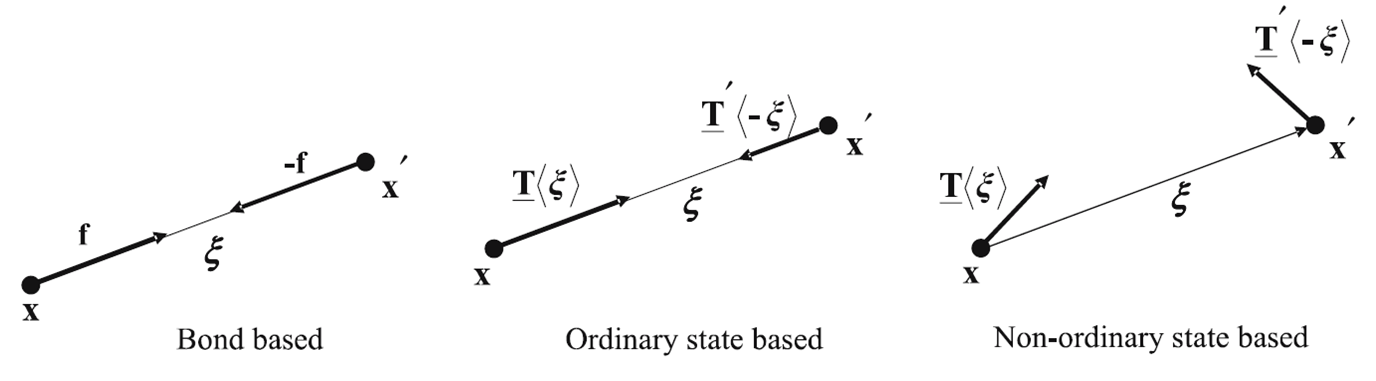
\includegraphics[width=\linewidth]{chap/image/peridynamics_models}

  \caption{\label{peridynamics_models}
           bond-based, ordinary state-based, non-ordinary state-based 模型对比示意图。在 bond-based 模型中,粒子之间彼此施加的力相等,且沿两者直线方向,因此本质上是质点弹簧系统。在 ordinary state-based 模型中,力沿两者直线方向,但彼此施加的力不一定相等。在 non-ordinary 模型中,对力的大小和方向并无约束,但需遵守动量和角动量守恒规律。图片取自\mycite{Silling}{2007}。
          }
\end{figure}

虽然近场动力学理论被倾向于用于处理线性弹性材料,但随着近场动力学理论的不断发展,学术界和工业界越来越意识到其理论优越性,其潜力也被不断挖掘。本文工作和其他实践证明其同样可以适用于处理非线性弹性、塑性、粘滞弹性、粘滞塑性等材料。限于本文篇幅,在此不能对近场动力学进行完整地阐述,更详细的介绍请参见\mycite{Madenci}{2014}。 本文工作所用的近场动力学模型基于 ordinary state-based 模型,但对原有理论进行了重新阐述以及修改,以适应图形学领域应用的特点。

\section{研究成果和创新点}

本文的主要研究成果是提出并实现了一种新的基于近场动力学理论的无网格框架来进行弹塑性物体的形变和碎裂仿真,其能够克服 FEM 在拓扑网格上面存在的困难,避免 remeshing 操作所引发的效率低下和实现复杂问题。在物理动力学上,其能够较为精确地仿真形变和碎裂行为,提供物理上和视觉上可信服的结果。此外,为表达弹塑性碎裂行为的视觉效果,本文还提出一种新的简单可用的嵌网格方法。本工作所提框架易于实现,并具有较强的可扩展性,在效率上相对于传统方法也更具优势。

具体而言,本文的创新点主要在于三点:
\begin{enumerate}
  \item 基于近场动力学理论,提出一种新的基于近场动力学理论无网格仿真框架。其支持包括弹塑性材料的弹性形变、塑性形变、弹塑性碎裂、脆性碎裂等多种复杂物理行为,同时能够很好地解决在 FEM 中不连续性引起的奇异值问题,避免复杂耗时的 remeshing 操作。此外,本文还对模型进行进一步扩展,使其能够支持简单的各向异性行为。
  \item 设计一种简单有效的嵌网格方法,所设计策略能够从几何表示上对物体的形变和碎裂行为进行追踪,能用于后续的碰撞处理以及提供高质量网格以用于渲染。本文力图所提的嵌网格方法是有效,完备的,可应用于其他无网格框架,且具有良好的扩展性。
  \item 基于 Physika\footnote{http://github.com/PhysikaTeam/Physika} 物理引擎,设计并实现相应的模型和主要算法,并对实现进行大量的实验和验证工作,和已有方法(FEM)进行充分对比。
\end{enumerate}

\section{本文组织结构}
本文主要分为六章。

第一章主要是本文工作的研究背景,介绍基于物理的仿真包括形变和碎裂仿真的研究意义以及在各领域的应用需求情况。梳理关于形变仿真、碎裂仿真、近场动力学的相关工作,同时明确本文的研究问题,介绍本文的研究成果和工作的创新点。

第二章概述性地介绍了物理仿真的基本原理,以及碎裂仿真的基本流程。并针对碎裂仿真中的三个主要要素,本构模型、碎裂模型、和离散时间积分在仿真中所扮演角色和作用,进行了一般性地介绍。最后针对近场动力学方法(PDM)的基本特征和本构方程基本形式,以及从经典连续介质力学到近场动力学的模型推导,作了较为详细的阐述。

第三章主要研究基于近场动力学理论的形变体仿真。全章首先重新表述了全文工作所用的弹塑性本构模型,并详细介绍了对应的离散化框架以及嵌网格策略。最后利用全章所述模型和方法,通过多样化材料的材质属性,对不同材料的形变行为进行模拟,展示相应的实验结果,并和 FEM 进行了充分的对比。

第四章主要研究基于近场动力学理论的碎裂仿真。在第三章的基础上,全章首先介绍了全文所用的碎裂模型,并对原有本构模型进行扩展,以支持简单的各向异性的碎裂行为。接着在已有离散框架上,详细介绍了拓扑网格更新方法以显式追踪碎裂带来的物体边界改变。最后展示了基于所述方法所取得的结果,实验证明本文所提方法能够高逼真地仿真弹脆性碎裂以及塑性碎裂。

第五章是对全文的工作总结和展望。


